\newpage

\subsection*{Codificación de línea, banda base}
Supongamos por ahora pulsos rectangulares. Algunos códigos de
línea son:

\FloatBarrier

\begin{ejemplo}$\phantom{1}$
    \FloatBarrier

    \begin{figure}[htb]
        \centering\begin{minipage}{\textwidth}
        \bpgf{Imagenes/codLinBB/codLinBB-1}
        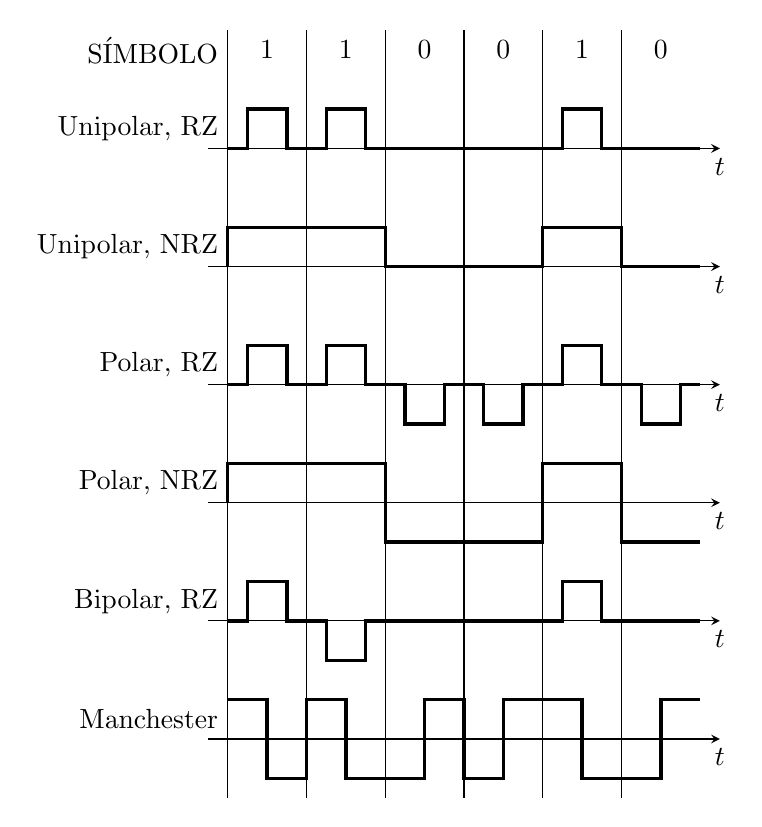
\begin{tikzpicture}[scale=0.5]
            \draw (0,1) -- (0,-18.5);
            \draw (2,1) -- (2,-18.5);
            \draw (4,1) -- (4,-18.5);
            \draw (6,1) -- (6,-18.5);
            \draw (8,1) -- (8,-18.5);
            \draw (10,1) -- (10,-18.5);
            \path (0,0.5) node [anchor=east] {SÍMBOLO} -- (1,0.5) node {$1$} -- (3,0.5) node {$1$} -- (5,0.5) node {$0$} -- (7,0.5) node {$0$} -- (9,0.5) node {$1$} -- (11,0.5) node {$0$};
            \begin{scope}[shift={(0,-2)}]
                \draw[-stealth] (-0.5,0) -- (12.5,0) node [anchor=north] {$t$};
                \path (0,0.5) node [anchor=east] {Unipolar, RZ};
                \draw[very thick] (0,0) -- (0.5,0) -- (0.5,1) -- (1.5,1) -- (1.5,0) -- (2.5,0) -- (2.5,1) -- (3.5,1) -- (3.5,0) -- (8.5,0) -- (8.5,1) -- (9.5,1) -- (9.5,0) -- (12,0);
            \end{scope}
            \begin{scope}[shift={(0,-5)}]
                \draw[-stealth] (-0.5,0) -- (12.5,0) node [anchor=north] {$t$};
                \path (0,0.5) node [anchor=east] {Unipolar, NRZ};
                \draw [very thick] (0,0) -- (0,1) -- (4,1) -- (4,0) -- (8,0) -- (8,1) -- (10,1) -- (10,0) -- (12,0);
            \end{scope}
            \begin{scope}[shift={(0,-8)}]
                \draw[-stealth] (-0.5,0) -- (12.5,0) node [anchor=north] {$t$};
                \path (0,0.5) node [anchor=east] {Polar, RZ};
                \draw [very thick] (0,0) -- (0.5,0) -- (0.5,1) -- (1.5,1) -- (1.5,0) -- (2.5,0) -- (2.5,1) -- (3.5,1) -- (3.5,0) -- (4.5,0) -- (4.5,-1) -- (5.5,-1) -- (5.5,0) -- (6.5,0) -- (6.5,-1) -- (7.5,-1) -- (7.5,0)-- (8.5,0) -- (8.5,1) -- (9.5,1) -- (9.5,0) -- (10.5,0) -- (10.5,-1) -- (11.5,-1) -- (11.5,0) -- (12,0);
            \end{scope}
            \begin{scope}[shift={(0,-11)}]
                \draw[-stealth] (-0.5,0) -- (12.5,0) node [anchor=north] {$t$};
                \path (0,0.5) node [anchor=east] {Polar, NRZ};
                \draw [very thick] (0,0) -- (0,1) -- (4,1) -- (4,-1) -- (8,-1) -- (8,1) -- (10,1) -- (10,-1) -- (12,-1);
            \end{scope}
            \begin{scope}[shift={(0,-14)}]
                \draw[-stealth] (-0.5,0) -- (12.5,0) node [anchor=north] {$t$};
                \path (0,0.5) node [anchor=east] {Bipolar, RZ};
                \draw[very thick] (0,0) -- (0.5,0) -- (0.5,1) -- (1.5,1) -- (1.5,0) -- (2.5,0) -- (2.5,-1) -- (3.5,-1) -- (3.5,0) -- (8.5,0) -- (8.5,1) -- (9.5,1) -- (9.5,0) -- (12,0);
            \end{scope}
            \begin{scope}[shift={(0,-17)}]
                \draw[-stealth] (-0.5,0) -- (12.5,0) node [anchor=north] {$t$};
                \path (0,0.5) node [anchor=east] {Manchester};
                \draw[very thick] (0,1) -- (1,1) -- (1,-1) -- (2,-1) -- (2,1) -- (3,1) -- (3,-1) -- (5,-1) -- (5,1) -- (6,1) -- (6,-1) -- (7,-1) -- (7,1) -- (9,1) -- (9,-1) -- (11,-1) -- (11,1) -- (12,1);
            \end{scope}
        \end{tikzpicture}
        \endpgfgraphicnamed\end{minipage}
    \end{figure}

\end{ejemplo}

\begin{ejemplo}[código cuaternario (polar)] 4 símbolos
    \begin{center}\begin{minipage}{\textwidth}
        \bpgf{Imagenes/codLinBB/codLinBB-2}
        \begin{tikzpicture}
            \draw (0,0) -- (0.5,0) -- (0.5,1.5) node [anchor=south east] {$3\,V$} -- (1.5,1.5) -- (1.5,0) -- (2,0);
            \draw (3,0) -- (3.5,0) -- (3.5,0.5) -- (4.5,0.5) node [anchor=south west] {$1\,V$} -- (4.5,0) -- (5,0);
            \draw (6,0) -- (6.5,0) -- (6.5,-0.5) node [anchor=north east] {$-1\,V$} -- (7.5,-0.5) -- (7.5,0) -- (8,0);
            \draw (9,0) -- (9.5,0) -- (9.5,-1.5) node [anchor=north east] {$-3\,V$} -- (10.5,-1.5) -- (10.5,0) -- (11,0);
        \end{tikzpicture}

        \endpgfgraphicnamed\end{minipage}
    \end{center}

%La codificación de línea afecta el espectro de la señal y por lo tanto su adecuación al canal.
\end{ejemplo}

La codificación de línea afecta muchas cosas:
\begin{itemize}
    \item Contenido de frecuencia de la señal, ¿tiene contínua?
    \item Extracción del reloj de sincronismo.
    \item Potencia requerida.
    \item Probabilidad de error de detección en presencia de ruido.
    \item Posibilidad de corrección de errores mediante redundancia.
\end{itemize}

\section{Densidad espectral de potencia de la señal PAM}\label{sec.densdig}

Consideramos la onda PAM (tren de pulsos modulados en amplitud)
\[
x(t) = \displaystyle\sum_k a_k p(t-kT_s).
\]
En general es difícil calcular el espectro ``de voltaje'', o sea
la transformada de Fourier de la propia señal, dado que depende de
la sucesión de símbolos que es en principio arbitraria.
Daremos sin embargo una expresión para el espectro \emph{de potencia}
de la señal PAM en función de la estadística del proceso de proceso de símbolos, y
de la forma del pulso.

Recordamos que en la Sección \ref{sec.estoc} ya se un analizó un ejemplo de este tipo: la ``onda binaria
aleatoria'' obtenida por símbolos independientes, idénticamente distribuidos (I.I.D.), $a_k=\pm 1$,
y pulsos $p(t)=p_{[0,T_s]}(t)$. Es decir, una onda PAM con codificación de línea polar,
NRZ. Interesa generalizar el estudio a otros pulsos y otras estadísticas de
símbolos.

El caso más utilizado es el siguiente: los símbolos siguen siendo I.I.D., pero con cualquier
distribución de probabilidad con media $E[a_k]=\mu$, y varianza $E[a_k^2]- \mu^2 = \sigma^2$.
El pulso $p(t)$ puede ser cualquiera de energía finita, con transformada de Fourier $\hat{P}(f)$.
 La fórmula para la densidad de potencia de la onda PAM es

\begin{center}
\col{S_x(f) = \sigma^2 f_s \left|\hat{P}(f)\right|^2 + \mu^2 f_s^2 \sum_{n=-\infty}^{+\infty}\left|\hat{P}(nf_s)\right|^2 \delta(f-nf_s)}
\end{center}

Remitimos al Apéndice \ref{appendix:pam} de estas notas para una demostración de esta fórmula, incluyendo una generalización a procesos de símbolos no necesariamente independientes. Una precisión es que para invocar la teoría de procesos estacionarios, es necesario (como en la Sección \ref{sec.estoc}) agregar a la onda un retardo aleatorio. No proseguiremos con este punto.

Analizamos lo que dice la fórmula anterior para el caso de pulsos NRZ.

\begin{ejemplo}[pulso NRZ]
    $p(t)=\begin{cases}
            1 & \text{si } 0 \leq t \leq T_s\\
            0 & \text{en otro caso}
          \end{cases}$, $\left|\hat{P}(f)\right|^2=T_s^2\sinc^2(\pi T_s f)$.

Notar que en este caso $\hat{P}(nf_s)=0$ para todo $n\neq 0$, por lo tanto el resultado es

\[S_x(f) = \sigma^2 T_s \sinc^2 (\pi T_s f) + \mu^2\delta(f).\]

    \begin{center}\begin{minipage}{\textwidth}
        \bpgf{Imagenes/codLinBB/codLinBB-3}
        \begin{tikzpicture}
            \draw [-stealth] (-6,0) -- (6,0) node [anchor=north] {$f$};
            \draw [-stealth] (0,-0.5) -- (0,4) node [anchor=east] {$S_x(f)$};
            \draw [samples=200,domain=-5:5] plot (\x,{2*(sin(3*\x r)/(3*\x))^2});
            \path (0,2) node [anchor=west] {$\sigma^2 T_s$};
            \path (-pi/3,0) node [anchor=north] {$-f_s$} -- (pi/3,0) node [anchor=north] {$f_s$} -- (2*pi/3,0) node [anchor=north] {$2 f_s$};
            \draw [very thick, -stealth] (0,0) -- (0,3.5) node [anchor=west] {$\mu^2$};
        \end{tikzpicture}
        \endpgfgraphicnamed\end{minipage}
    \end{center}

Si particularizamos al caso de la onda binaria aleatoria, $a_k=\pm 1$, I.I.D., tenemos
 $\mu=0$, $\sigma^2=1$, por lo tanto reencontramos el resultado hallado anteriormente.
 \end{ejemplo}



\subsection*{¿Qué conclusiones podemos sacar de $S_x(f)$?}

\begin{enumerate}
    \item Potencia total: $\langle x^2\rangle = \displaystyle\int_{-\infty}^{\infty} S_x(f)\d f $.
    En el ejemplo de pulsos NRZ,
    \[
     \langle x^2\rangle = \mu^2 +\sigma^2 f_s \displaystyle\int_{-\infty}^{\infty}
    \left|\hat{P}(f)\right|^2\d f = \mu^2 +\sigma^2 f_s \displaystyle\int_{-\infty}^{\infty} \left|p(t)\right|^2\d
    t = \mu^2 + \sigma^2.\]
    \item Porcentaje de potencia dentro de una banda.  Ver más abajo.
     \item Valor de continua. En el caso NRZ, si la señalización es:
    \begin{itemize}
        \item unipolar, $a_k\in \{0,A\}\Rightarrow \mu=\frac{A}{2}$, hay continua.
        \item polar, $a_k\in \{-A,A\}\Rightarrow \mu = 0$, no hay continua.
    \end{itemize}
    \item \emph{Sincronismo}: para poder sacar ``el reloj'' de la señal debería haber un $\delta$ en $f_s$ o algún múltiplo. Por lo tanto, la onda PAM con pulsos NRZ
     no provee sincronismo.
\end{enumerate}
\newpage

\begin{ejemplo}
    Veamos el caso de pulso RZ.\begin{minipage}{5cm}
                                \bpgf{Imagenes/codLinBB/codLinBB-4}
                                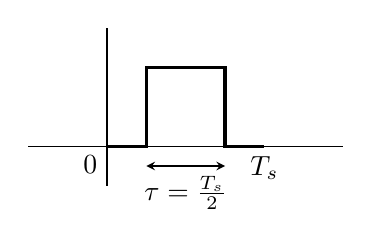
\begin{tikzpicture}[xscale=2]
                                    \draw (-0.5,0) -- (1.5,0);
                                    \draw (0,-0.5) -- (0,1.5);
                                    \path (0,0) node [anchor=north east] {$0$} -- (1,0) node [anchor=north] {$T_s$};
                                    \draw [very thick] (0,0) -- (0.25,0) -- (0.25,1) -- (0.75,1) -- (0.75,0) -- (1,0);
                                    \draw [stealth-stealth] (0.25,-0.25) -- (0.75,-0.25);
                                    \path (0.5,-0.25) node [anchor=north] {$\tau=\frac{T_s}{2}$};
                                \end{tikzpicture}
                                \endpgfgraphicnamed%\end{minipage}
                               \end{minipage}

    \[\left|\hat{P}(f)\right|^2=\left(\frac{T_s}{2}\right)^2 \sinc^2\left(\pi f \frac{T_s}{2}\right)\]

    \begin{center}\begin{minipage}{\textwidth}
        \bpgf{Imagenes/codLinBB/codLinBB-5}
        \begin{tikzpicture}
            \draw [-stealth] (-6,0) -- (6,0) node [anchor=north] {$f$};
            \draw [-stealth] (0,-0.5) -- (0,5) node [anchor=east] {$S_x(f)$};
            \draw [samples=200,domain=-5:5] plot (\x,{4*(sin(3*\x/2 r)/(3*\x/2))^2});
            \path (0,4) node [anchor=west] {$\frac{\sigma^2 T_s}{4}$};
            \path (-pi,0) node [anchor=north] {$-3 f_s$} -- (-2*pi/3,0) node [anchor=north] {$-2 f_s$} -- (-pi/3,0) node [anchor=north] {$-f_s$} -- (pi/3,0) node [anchor=north] {$f_s$} -- (2*pi/3,0) node [anchor=north] {$2 f_s$} -- (pi,0) node [anchor=north] {$3 f_s$};
            \draw [very thick, -stealth] (0,0) -- (0,2.5) node [anchor=west] {$\frac{\mu^2}{4}$};
            \draw [very thick,-stealth] (-pi,0) -- (-pi,0.25);
            \draw [very thick,-stealth] (-pi/3,0) -- (-pi/3,1);
            \draw [very thick,-stealth] (pi/3,0) -- (pi/3,1);
            \draw [very thick,-stealth] (pi,0) -- (pi,0.25);
        \end{tikzpicture}
        \endpgfgraphicnamed\end{minipage}
    \end{center}

    Aquí sí hay información de sincronismo para $\mu\neq 0$.
\end{ejemplo}

\paragraph{Pregunta} ¿Qué porcentaje de la energía de un pulso rectangular entra en las distintas bandas?

Sea $p(t)$  \begin{minipage}{5cm}
        \bpgf{Imagenes/codLinBB/codLinBB-6}
        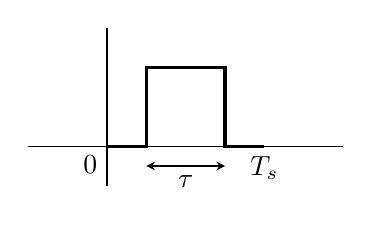
\begin{tikzpicture}[xscale=2]
            \draw (-0.5,0) -- (1.5,0);
            \draw (0,-0.5) -- (0,1.5);
            \path (0,0) node [anchor=north east] {$0$} -- (1,0) node [anchor=north] {$T_s$};
            \draw [very thick] (0,0) -- (0.25,0) -- (0.25,1) -- (0.75,1) -- (0.75,0) -- (1,0);
            \draw [stealth-stealth] (0.25,-0.25) -- (0.75,-0.25);
            \path (0.5,-0.25) node [anchor=north] {$\tau$};
        \end{tikzpicture}
        \endpgfgraphicnamed
        \end{minipage} con área $1$. $|\hat{P}(f)| = |\sinc (\pi \tau f)|$

\begin{minipage}{0.45\textwidth}
    \bpgf{Imagenes/codLinBB/codLinBB-7}
        \begin{tikzpicture}
            \draw [-stealth] (-0.5,0) -- (6,0) node [anchor=north] {$f$};
            \draw [-stealth] (0,-0.5) -- (0,5) node [anchor=west] {$\sinc^2(\pi \tau f)$};
            \draw [samples=200,domain=0.001:5] plot (\x,{4*(sin(3*\x/2 r)/(3*\x/2))^2});
            \path (0,4) node [anchor=east] {$1$};
            \draw (pi/3,0) node [anchor=north] {$\frac{1}{2\tau}$} -- (pi/3,{4*(sin(pi/2 r)/(pi/2))^2});
            \path (2*pi/3,0) node [anchor=north] {$\frac{1}{\tau}$} -- (4*pi/3,0) node [anchor=north] {$\frac{2}{\tau}$};
        \end{tikzpicture}
    \endpgfgraphicnamed
\end{minipage}
\begin{minipage}{0.2\textwidth}
    \begin{tabular}{c|c}
        $\tau f$ & \% pot\\
        \hline
        $\tfrac{1}{2}$ & $77$\\
        $1$ & $90$\\
        $2$ & $95$\\
        $3$ & $96.6$\\
        $\vdots$ & \\
        $11$ & $99$
    \end{tabular}
\end{minipage}
\begin{minipage}{0.25\textwidth}
    Se usa muchas veces $B=\tfrac{1}{\tau}$ como ancho de banda práctico.
\end{minipage}


\paragraph{Interpretación de la fórmula}

\begin{equation}
    \label{eq:dig2}S_x(f) = \sigma^2 f_s \left|\hat{P}(f)\right|^2 + \mu^2 f_s^2 \sum_{n=-\infty}^{+\infty} \left|\hat{P}(nf_s)\right|^2\delta(f-nf_s)\tag{\textasteriskcentered}
\end{equation}
Escribamos la onda PAM como superposición de dos términos:
\[x(t)= \underbrace{\sum_k (a_k-\mu) p(t-kT_s)}_{\text{aleatorio, media $0$}} +  \underbrace{\mu\sum_k p(t-kT_s)}_{\text{periódico, $z(t)$}}.\]
Analizamos por Fourier el término periódico:
\begin{align*}
    z(t) & = \mu \cdot p(t) \ast \sum_k \delta(t-kT_s)  \\
    \Rightarrow \hat{Z}(f)  & = \mu \hat{P}(f) f_s \sum_n \delta(f-nf_s) = \sum_n \mu f_s \hat{P}(nf_s) \delta(f-nf_s),
\end{align*}
de donde obtenemos la siguiente serie de Fourier:
\begin{align*}%\label{serfouz}
z(t) = \sum_n \mu f_s \hat{P}(nf_s)\e^{jn\omega_s t}.
\end{align*}
La densidad espectral de potencia de esta superposición de sinusoides es
\[S_z(f) = \sum_n \mu^2 f_s^2\left|\hat{P}(nf_s)\right|^2 \delta(f-nf_s) = \text{2º término de \eqref{eq:dig2}}.\]
Es decir que los dos términos del espectro de potencia  \eqref{eq:dig2} se interpretan como:
\begin{itemize}
    \item Un espectro continuo, que representa la parte aleatoria, con media $0$.
    \item Un espectro discreto que representa la parte determinística, periódica.
\end{itemize}


\newpage

\subsection*{Potencia de la señal digital}

Integrando la expresión \eqref{eq:dig2} en frecuencia, tenemos
\begin{align*} \langle x^2 \rangle &= \sigma^2
f_s\displaystyle\int_{-\infty}^{+\infty}\left|\hat{P}(f)\right|^2\d
f + \langle z^2\rangle \\
& = \sigma^2 \|p\|^2 f_s +\langle z^2\rangle.
\end{align*}

Aquí  $\|p\|^2 = \displaystyle\int_{-\infty}^{+\infty} p(t)^2\d t$
es la energía del pulso $p(t)$.
%
%    \begin{center}
%        \col{\langle x^2\rangle  } Potencia de señal digital.
%    \end{center}

También se acostumbra definir la \emph{energía media} del pulso aleatorio $a_k p(t-kT_s)$,
que esta dada por
\begin{align*}
    \overline{E_p} = E[a_k^2] \|p\|^2  = (\mu^2+ \sigma^2)\|p\|^2 .
\end{align*}


\noindent Hay algunos casos particulares en que la parte periódica cumple  $\langle
z^2\rangle = \mu^2 \|p\|^2 f_s$. En este caso, tendremos:
\begin{align*}
    \langle x^2\rangle  & = \overline{E_p} f_s,
\end{align*}
fórmula con interpretación intuitiva: envío un pulso de energía media $\overline{E_p}$, cada $T_s$ segundos,
la potencia media es $\overline{E_p}/T_s = \overline{E_p} f_s$. Sin embargo, para que esta interpretación sea válida es necesario que los pulsos
sucesivos sean ortogonales entre sí, lo cual se cumple sólo en algunos casos, como detallamos a continuación.


Validez de la fórmula $\langle x^2\rangle  =
{\overline{E_p}}{f_s}$:
\begin{itemize}
    \item Siempre que $\mu=0$, o sea $x(t)$ es una señal polar. Aquí la parte periódica desaparece.
    \item El pulso $p(t)$ tiene duración menor o igual a $T_s$.
    \item Los pulsos son de Nyquist ideales (definidos más adelante).
\end{itemize}

Para ver el segundo caso: si $p(t)$ tiene soporte en
$[0,T_s]\Rightarrow \mu p(t)$ es un período de $z(t)$
\[\Rightarrow \langle z^2\rangle  = \frac{1}{T_s} \int_0^{T_s} z^2(t)\d t = \frac{\mu^2}{T_s}\int_0^{T_s} p(t)^2\d t=
 \mu^2
\|p\|^2 f_s.\]
Alternativamente, notar que en este caso los pulsos $p(t-kT_s)$ y $p(t-lT_s)$ son ortogonales para $k\neq l$, ya que no se solapan. Esta ortogonalidad también se cumplirá en el tercer caso, como se verá después.
